\section{Erhalt erster Integrale}

Betrachte die autonome Differentialgleichung $x'=f(x)$ auf einem Phasenraum $\Omega_0$.

\begin{definition}
	Eine Funktion $\mathcal E \colon \Omega_0 \to \R$ heißt \begriff{erstes Integral}, wenn
	\begin{equation*}
		\mathcal E(\Phi^t x) = \mathcal E(x)
	\end{equation*}
	für alle $x\in\Omega_0$ und alle zulässigen $t$ gilt.
\end{definition}

Alternative Bezeichnungen: Invariante, Erhaltungsgröße, engl.: constant of motion

\begin{bsp}
	Mathematisches (Faden-)pendel
	\begin{center}
		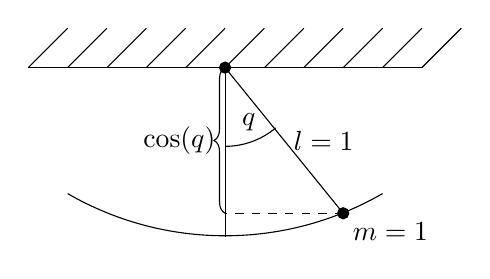
\begin{tikzpicture}
			\draw (0,4) -- (5,4);
			\foreach \i in {0,...,10}
			\draw (\i / 2, 4) -- ( \i/2+ 0.5, 4.5);
			\draw[fill] (2.5,4) circle (2pt);
			\draw[fill] (4,2.15) circle (2pt) node[below right]{$m=1$};
			\draw (0.5,2.4) arc (-120:-60:4);
			\draw  (2.5,4) -- node[right]{$l=1$} (4,2.15) ;
			\draw (2.5,4) -- (2.5,1.85);
			\draw[dashed] (4,2.15) -- (2.5,2.15);
			\draw (2.5, 3) arc (-90:-50:1);
			\draw (2.8,3.3) node {$q$};
			\draw [decorate,decoration={brace,amplitude=4pt}]
			(2.5,2.15)--(2.5,4) node[midway, left] {$\cos(q)$};
		\end{tikzpicture}
	\end{center}
	
	Bewegungsgleichungen für Winkel $q$:
	\begin{equation*}
		\ddot{q} + \frac{g}{l} \sin q = 0
	\end{equation*}
	bzw. als System erster Ordnung:
	\begin{equation*}
		\begin{aligned}
			\dot{p} &= - mgl \sin q\\
			\dot{q} &= \frac{1}{ml^2} p
		\end{aligned}
	\end{equation*}
	Erhält $\mathcal E(p,q) = \frac{1}{2} \frac{1}{ml^2} p^2 - mgl \cos q $ (die totale Energie).
\end{bsp}

\begin{bsp}
	Betrachte ein System mit $N$ Partikeln
	\begin{itemize}
		\item $q_i\in\R^3,\ i=1,\hdots,N$ Positionen, $p_i\in\R,\ i=1,\hdots,N$ Impulse
		\item $m_i$: Massen
		\item Paarweise Interaktion über Kräfte, die vom Abstand abhängen.
	\end{itemize}
	Bewegungsgleichungen:
	\begin{equation*}
	q_i'=\frac{p_i}{m_i},\qquad p_i' = \sum_{j=1}^N \nu_{ij}(q_i-q_j)
	\end{equation*}
	mit
	\begin{align*}
	\nu_{ij}(y) = - \nu_{ji}(-y)
	\end{align*}
	daraus folgt insbesondere dass $\nu_{ii} = 0$.
	
	Die Bewegungsgleichungen erhalten den Gesamtimpuls $P=\sum_{i=1}^Np_i$, denn
	\begin{equation*}
	\frac{d}{dt}\sum_{i=1}^Np_i = \sum_{i=1}^N p_i' = \sum_{i=1}^N\sum_{j=1}^N\nu_{ij}(q_i-q_j) = 0
	\end{equation*}
	Ebenso: Der Gesamtdrehimpuls $L=\sum_{i=1}^N q_i\times p_i$
	\begin{align*}
		\frac{d}{dt}\sum_{i=1}^N q_i\times p_i
		& = \sum_{i=1}^N q_i'\times p_i+\sum_{i=1}^N q_i\times p_i' \\
		& = \sum_{i=1}^N \frac{1}{m_i}\underbrace{p_i\times p_i}_{=0} + \sum_{i=1}^N\sum_{j=1}^Nq_i\times\nu_{ij}(q_i-q_j) \\
		& = 0.
	\end{align*}
\end{bsp}

Klassifikation der Erhaltungsgrößen: (für diese Beispiele)
\begin{itemize}
 \item Impuls: linear
 \item Drehimpuls: quadratisch
 \item Energie beim Fadenpendel: nichtlinear
\end{itemize}

Man hätte nun gerne numerische Verfahren, die erste Integrale erhalten.

Zunächst eine einfache Charakterisierung mit Hilfe von $f$:

\begin{lemma}[{{\cite[6.56]{deuflhard_bornemann:2008}}}]
	Sei $f$ lokal Lipschitz-stetig. Eine Funktion $\mathcal E\in C^1(\Omega_0,\R)$ ist genau dann erstes Integral, wenn
	\begin{equation*}
		\nabla\mathcal E(x)\cdot f(x) = 0
	\end{equation*}
	für alle $x\in\Omega_0$.
\end{lemma}
\begin{proof}
	Die Kettenregel liefert $\displaystyle 0 = \frac{d}{dt} \mathcal E(\Phi^t x) = \nabla\mathcal E(\Phi^tx)\cdot \frac{d}{dt}\Phi^tx = \nabla\mathcal E(\Phi^tx)\cdot f(\Phi^tx)$.
\end{proof}

\begin{bsp}
	Wir zeigen Energieerhaltung des Fadenpendels.
	Für dieses Modell gilt:
	\begin{align*}
		f(x) & = f(p,q)
		=
		\begin{pmatrix}
		- mgl \sin q \\ \frac{p}{ml^2}
		\end{pmatrix} \\
		%
		\mathcal{E}(x) & = \mathcal{E}(p,q)
		=
		\frac{1}{2} \frac{p^2}{ml^2} - mgl \cos q
	\end{align*}
	Der Gradient der Energie ist
	\begin{equation*}
		\nabla \mathcal{E}(p,q) =
		\begin{pmatrix}
		\frac{p}{ml^2} \\ mgl \sin q
		\end{pmatrix}
	\end{equation*}
	Damit erhält man
	\begin{equation*}
		\nabla \mathcal{E}(p,q) \cdot f(p,q)
		= \frac{p}{ml^2}(- mgl \sin q) + mgl \sin q\frac{p}{ml^2}
		= 0
	\end{equation*}
\end{bsp}


\begin{satz}[{{\cite[Thm.\ IV.1.5]{hairer_lubich_wanner:2006}}}]
	Alle Runge-Kutta-Verfahren erhalten lineare Invarianten.
\end{satz}
\begin{proof}%\mbox{}
	Sei $\mathcal{E}$ lineare Invariante, also $\mathcal{E}(x) = d^Tx$ mit festem Vektor $d$.
	Nach dem vorigen Satz ist dann $d^T f(x) = 0$ für alle $x\in\Omega_0$.
	Für eine Stufe $k_i$ eines beliebigen RK-Verfahrens ist dann
	\begin{equation*}
		d^T k_i = d^T f\Big( x+\tau\sum_{j=1}^s a_{ij}k_j \Big) = 0.
	\end{equation*}
	Also ist
	\begin{equation*}
		\mathcal E(x_{k+1})
		= d^T x_{k+1}
		= d^T\Big(x_k+\tau\sum_{i=1}^s b_{i}k_i\Big)
		= d^T x_k
		= \mathcal{E}(x_k)
	\end{equation*}
\end{proof}

Für die quadratischen Invarianten betrachten wir zunächst einen wichtigen Spezialfall:

\textbf{Frage:} Für welche linearen autonomen Differentialgleichungen $x' = Ax$ erhält der Phasenfluss $\Phi^t$ die Euklidische Norm $\norm{\Phi^t x}_2 = \norm{x}_2$ für alle $t$?
\textbf{Antwort:} Genau dann, wenn $\Phi^t = \exp(tA)$ eine orthogonale Matrix ist.
\begin{satz}[{{\cite[6.18]{deuflhard_bornemann:2008}}}]
\label{thm:normerhaltende_fluesse}
	Sei $A\in\R^{d \times d}$. Die Matrix $\exp(tA)$ ist genau dann orthogonal,
	wenn $A$ schiefsymmetrisch ist.
\end{satz}
\begin{proof}
	\begin{description}
		\item[($\boldsymbol{\Rightarrow}$)] Sei $\exp(tA)\in O(d)$ für alle $t$.
		Dann ist
		\begin{equation*}
			I = \exp(tA)^T \exp(tA) = \exp(tA^T) \exp(tA).
		\end{equation*}
		Differenziere nach $t$ und betrachte $t=0$
		\begin{equation*}
			0=\Big(A^T \exp(tA^T) \exp(tA) + \exp(tA^T)A \exp(tA) \Big)\Big|_{t=0} = A^T+A
		\end{equation*}
		\item[($\boldsymbol{\Leftarrow}$)] 
		\begin{align*}
			I
			&= \exp(tA-tA) = \exp(tA)\cdot \exp(-tA)\quad\text{(da $A$ mit $A$ kommutiert)}\\
			&= \exp(tA)\cdot \exp(tA^T) \\
			&= \exp(tA)\cdot \exp(tA)^T	 
		\end{align*}
	\end{description}
\end{proof}

Zentral ist anscheinend die Eigenschaft
\begin{equation*}
	\exp(z)\cdot \exp(-z) = 1\qquad \forall z\in\C.
\end{equation*}
Das nennt man \begriff{Reversibilität}.

Man hätte diese Eigenschaft gerne auch für diskrete Verfahren.
\begin{definition}
	Eine diskrete Evolution $\Psi$ heißt reversibel, wenn
	\begin{equation*}
		\Psi^{t,t+\tau}\Psi^{t+\tau,t} x = x
	\end{equation*}
	für alle $(t,x)\in\Omega$ und hinreichend kleine $\tau$.
\end{definition}

\begin{bsp}
	Das explizite Euler-Verfahren ist nicht reversibel.
\end{bsp}

Reversible rationale Approximationen der Exponentialfunktion erzeugen normerhaltende diskrete Flüsse.

\begin{satz}[{{\cite[6.21]{deuflhard_bornemann:2008}}}]
	Sei $R$ eine rationale, konsistente, reversible Approximation der Exponentialfunktion. Dann gilt für eine Matrix $A\in\R^{d\times d}$
	\begin{equation*}
		R(\tau A)\in O(d)\qquad\forall \tau > 0
	\end{equation*}
	genau dann, wenn $A=-A^T$.
\end{satz}
\begin{proof}
	Weitestgehend wie bei Satz~\ref{thm:normerhaltende_fluesse}.
\end{proof}

\begin{bsp}
	\begin{equation*}
		R(z) = \frac{1+\frac{z}{2}}{1-\frac{z}{2}}=1+z+\frac{z^2}{2} + \frac{z^3}{4} + \mathcal{O}(z^4) = e^z + \mathcal O(z^3)
	\end{equation*}
	\begin{itemize}
		\item Die entsprechende Matrix-Abbildung heißt \begriff{Cayley-Transformation}.
		\item Stabilitätsfunktion insbesondere der impliziten Mittelpunktsregel $\to$ dem einfachsten Gauß-Verfahren.
	\end{itemize}
	Gauß-Verfahren erhalten sogar beliebige quadratische Invarianten!
\end{bsp}

\begin{satz}[{{\cite[6.58]{deuflhard_bornemann:2008}}}]
	Die Differentialgleichung $x'=f(x)$ mit lokal Lipschitz-stetigem $f$ besitze das quadratische erste Integral $\mathcal E$, d.h.
	\begin{equation*}
		\mathcal E(x) = x^T E x + e^T x + \eta
	\end{equation*}
	mit $E\in\R^{d\times d},\ e\in\R^d,\ \eta\in\R$. Jedes Gaus-Verfahren erzeugt einen Phasenfluss $\Psi$, der $\mathcal E$ erhält, d.h.
	\begin{equation*}
		\mathcal E(\Psi^\tau x) = \mathcal E(x)
	\end{equation*}
	für alle $x\in\Omega_0$ und zulässige $\tau$.
\end{satz}
\begin{proof}
	Ganz ähnlich wie der Beweis der $B$-Stabilität.
	Sei $x\in\Omega_0$, und $\tau$ so klein, dass das Kollokationspolynom
	\begin{equation*}
		u\in P_s,\quad u(0)=x,\quad u(\tau) = \Psi^\tau x
	\end{equation*}
	existiert. Da $\mathcal E$ quadratisch ist, ist $q(\theta) \colonequals \mathcal E(u(\theta\tau))$ ein Polynom in $P_{2s}$.
	Der Hauptsatz der Integralrechnung liefert
	\begin{equation*}
		\mathcal E(\Psi^\tau x) = q(1) = q(0) + \int_0^1q'(\theta)\,d\theta = \mathcal E(x) + \int_0^1q'(\theta)\,d\theta . 
	\end{equation*}
	Zu zeigen ist nun also $\int_0^1q'(\theta)\,d\theta =0$.
	Nutze die Quadraturformel des Gauß-Verfahrens. Diese ist für Polynome in $P_{2s-1}$ exakt:
	\begin{equation*}
		\int_0^1q'(\theta)\,d\theta = \sum_{j=1}^s b_j q'(c_j).
	\end{equation*}
	Es sind aber alle $q'(c_j)=0$, denn
	\begin{align*}
		q'(c_j) 
		&= \big(\mathcal E(u(c_j\tau))\big)' \\
		&= \tau\nabla\mathcal E(u(c_j\tau))\cdot u'(c_j\tau) \tag{Kettenregel} \\
		&= \tau\nabla\mathcal E(u(c_j\tau))\cdot f(u(c_j\tau)) \tag{Kollokationseigenschaft} \\
		&= 0 \tag{da $\mathcal E$ eine Invariante ist}
	\end{align*}
\end{proof}

Was ist mit der Energieerhaltung des Fadenpendels? $\to$ Das behandeln wir später mit der Theorie der Hamiltonschen Systeme.